% Approach overview figure. Compile on its own (pdflatex approach_overview.tex) to get
% approach_overview.pdf, which the paper includes with \includegraphics.
\documentclass[tikz,border=4pt]{standalone}
\usepackage[scaled=0.92]{helvet}
\renewcommand{\familydefault}{\sfdefault}
\usetikzlibrary{positioning,fit,backgrounds,shapes.geometric,arrows.meta,calc}

\definecolor{ink}{HTML}{1F2933}
\definecolor{sub}{HTML}{52606D}
\definecolor{fillA}{HTML}{EEF2F7}
\definecolor{fillB}{HTML}{FFF4E5}
\definecolor{edge}{HTML}{3E4C59}
\definecolor{accent}{HTML}{A61C3C}
\definecolor{panel}{HTML}{F7F8FA}

\tikzset{
  nohyph/.style={execute at begin node={\hyphenpenalty=10000\exhyphenpenalty=10000}},
  box/.style={nohyph, draw=edge, line width=0.5pt, rounded corners=2pt, fill=fillA,
              text width=2.30cm, minimum height=1.15cm, align=center, inner sep=2.5pt,
              font=\fontsize{6.6}{7.7}\selectfont\color{ink}},
  hum/.style={box, fill=fillB},
  db/.style={nohyph, cylinder, shape border rotate=90, aspect=0.18, draw=edge, line width=0.5pt,
             fill=white, text width=1.50cm, minimum height=1.15cm, align=center, inner sep=1.5pt,
             font=\fontsize{6.6}{7.7}\selectfont\color{ink}},
  rqout/.style={box, fill=white, draw=accent, line width=0.8pt, text width=1.50cm},
  future/.style={box, fill=white, dashed, text width=1.50cm},
  arr/.style={-{Stealth[length=4.2pt,width=3.6pt]}, line width=0.6pt, draw=edge},
  link/.style={-{Stealth[length=4.6pt,width=4pt]}, line width=0.8pt, draw=accent, rounded corners=3pt},
  lbl/.style={font=\fontsize{5.8}{6.6}\selectfont\itshape\color{accent}, inner sep=1.5pt},
  panelbox/.style={draw=sub, dashed, line width=0.5pt, rounded corners=3pt, fill=panel,
                   inner xsep=6pt, inner ysep=6pt},
  tab/.style={draw=ink, fill=white, line width=0.6pt, font=\fontsize{7.2}{8}\selectfont\bfseries,
              inner sep=2.5pt, anchor=west},
}
\newcommand{\st}[2]{\textbf{#1}\\[1pt]{\color{sub}#2}}
\newcommand{\rowgap}{2.45}

\begin{document}
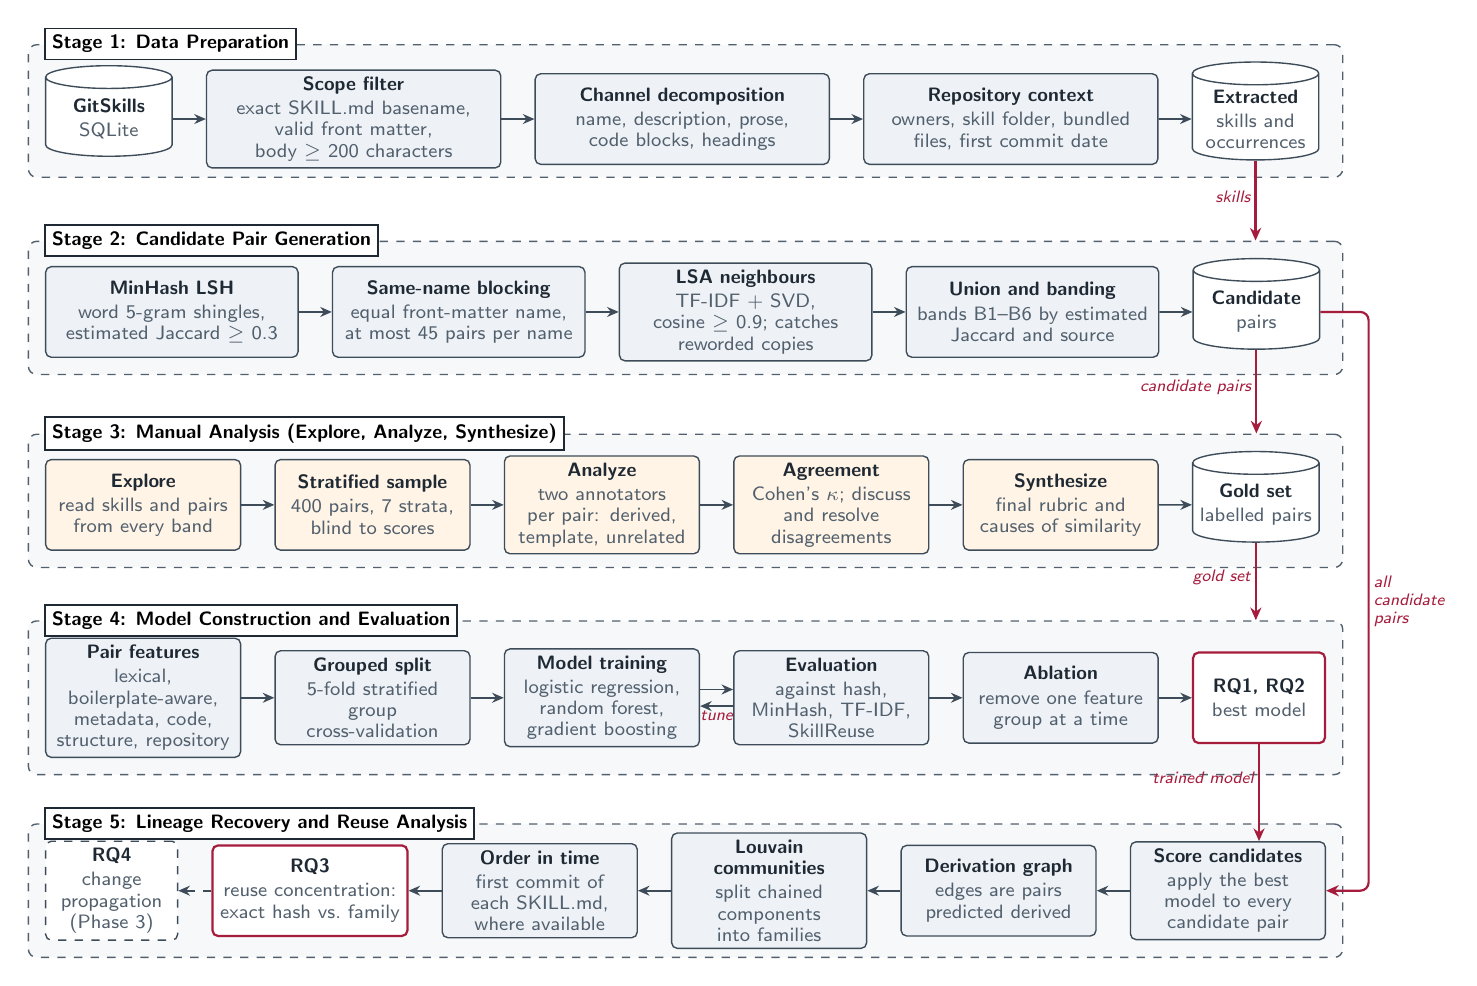
\begin{tikzpicture}[node distance=0.42cm]

% ---------- Stage 1 (row y=0) ----------
\node[db, anchor=west] (gs) at (0,0) {\textbf{GitSkills}\\[1pt]{\color{sub}SQLite}};
\node[box, right=of gs, text width=3.56cm] (scope) {\st{Scope filter}{exact SKILL.md basename, valid front matter, body $\geq$ 200 characters}};
\node[box, right=of scope, text width=3.56cm] (dec) {\st{Channel decomposition}{name, description, prose, code blocks, headings}};
\node[box, right=of dec, text width=3.56cm] (ctx) {\st{Repository context}{owners, skill folder, bundled files, first commit date}};
\node[db, right=of ctx] (xdb) {\textbf{Extracted}\\[1pt]{\color{sub}skills and occurrences}};
\foreach \a/\b in {gs/scope, scope/dec, dec/ctx, ctx/xdb} \draw[arr] (\a) -- (\b);

% ---------- Stage 2 ----------
\node[box, anchor=west, text width=3.03cm] (lsh) at (0,-\rowgap) {\st{MinHash LSH}{word 5-gram shingles, estimated Jaccard $\geq$ 0.3}};
\node[box, right=of lsh, text width=3.03cm] (name) {\st{Same-name blocking}{equal front-matter name, at most 45 pairs per name}};
\node[box, right=of name, text width=3.03cm] (lsa) {\st{LSA neighbours}{TF-IDF + SVD, cosine $\geq$ 0.9; catches reworded copies}};
\node[box, right=of lsa, text width=3.03cm] (band) {\st{Union and banding}{bands B1--B6 by estimated Jaccard and source}};
\node[db, right=of band] (cand) {\textbf{Candidate}\\[1pt]{\color{sub}pairs}};
\foreach \a/\b in {lsh/name, name/lsa, lsa/band, band/cand} \draw[arr] (\a) -- (\b);

% ---------- Stage 3 ----------
\node[hum, anchor=west] (exp) at (0,-2*\rowgap) {\st{Explore}{read skills and pairs from every band}};
\node[hum, right=of exp] (samp) {\st{Stratified sample}{400 pairs, 7 strata, blind to scores}};
\node[hum, right=of samp] (lab) {\st{Analyze}{two annotators per pair: derived, template, unrelated}};
\node[hum, right=of lab] (kap) {\st{Agreement}{Cohen's $\kappa$; discuss and resolve disagreements}};
\node[hum, right=of kap] (syn) {\st{Synthesize}{final rubric and causes of similarity}};
\node[db, right=of syn] (gold) {\textbf{Gold set}\\[1pt]{\color{sub}labelled pairs}};
\foreach \a/\b in {exp/samp, samp/lab, lab/kap, kap/syn, syn/gold} \draw[arr] (\a) -- (\b);

% ---------- Stage 4 ----------
\node[box, anchor=west] (feat) at (0,-3*\rowgap) {\st{Pair features}{lexical, boilerplate-aware, metadata, code, structure, repository}};
\node[box, right=of feat] (cv) {\st{Grouped split}{5-fold stratified group cross-validation}};
\node[box, right=of cv] (clf) {\st{Model training}{logistic regression, random forest, gradient boosting}};
\node[box, right=of clf] (eval) {\st{Evaluation}{against hash, MinHash, TF-IDF, SkillReuse}};
\node[box, right=of eval] (abl) {\st{Ablation}{remove one feature group at a time}};
\node[rqout, right=of abl] (rq12) {\textbf{RQ1, RQ2}\\[1pt]{\color{sub}best model}};
\foreach \a/\b in {feat/cv, cv/clf, eval/abl, abl/rq12} \draw[arr] (\a) -- (\b);
\draw[arr] ([yshift=3pt]clf.east) -- ([yshift=3pt]eval.west);
\draw[arr] ([yshift=-3pt]eval.west) -- ([yshift=-3pt]clf.east);
\node[lbl, below=0pt of $(clf.east)!0.5!(eval.west)$, yshift=-3pt] {tune};

% ---------- Stage 5 (reads right to left: inputs arrive on the right) ----------
\coordinate (R0) at ($(rq12.east)+(0,-\rowgap)$);
\node[box, anchor=east] (score) at (R0) {\st{Score candidates}{apply the best model to every candidate pair}};
\node[box, left=of score] (graph) {\st{Derivation graph}{edges are pairs predicted derived}};
\node[box, left=of graph] (lou) {\st{Louvain communities}{split chained components into families}};
\node[box, left=of lou] (ord) {\st{Order in time}{first commit of each SKILL.md, where available}};
\node[rqout, left=of ord, text width=2.30cm] (conc) {\st{RQ3}{reuse concentration: exact hash vs.\ family}};
\node[future, left=of conc] (rq4) {\st{RQ4}{change propagation (Phase 3)}};
\foreach \a/\b in {score/graph, graph/lou, lou/ord, ord/conc} \draw[arr] (\a) -- (\b);
\draw[arr, dashed] (conc) -- (rq4);

% ---------- panels (common left and right edges) ----------
\coordinate (R) at (rq12.east);
\begin{scope}[on background layer]
  \foreach \p/\a/\b in {p1/gs/xdb, p2/lsh/cand, p3/exp/gold, p4/feat/rq12, p5/rq4/score}{
    \node[panelbox, fit=(\a)(\b)(\a.west |- \a.north)(R |- \b.south)] (\p) {};
  }
\end{scope}
\node[tab] at ([xshift=6pt]p1.north west) {Stage 1: Data Preparation};
\node[tab] at ([xshift=6pt]p2.north west) {Stage 2: Candidate Pair Generation};
\node[tab] at ([xshift=6pt]p3.north west) {Stage 3: Manual Analysis (Explore, Analyze, Synthesize)};
\node[tab] at ([xshift=6pt]p4.north west) {Stage 4: Model Construction and Evaluation};
\node[tab] at ([xshift=6pt]p5.north west) {Stage 5: Lineage Recovery and Reuse Analysis};

% ---------- data flow between stages (right-hand side, clear of the tabs) ----------
\draw[link] (xdb.south) -- (xdb.south |- p2.north) node[lbl, pos=0.45, left] {skills};
\draw[link] (cand.south) -- (cand.south |- p3.north) node[lbl, pos=0.45, left] {candidate pairs};
\draw[link] (gold.south) -- (gold.south |- p4.north) node[lbl, pos=0.45, left] {gold set};
\draw[link] (rq12.south) -- (rq12.south |- score.north) node[lbl, pos=0.35, left] {trained model};
\coordinate (gut) at ($(p1.east)+(0.32,0)$);
\draw[link] (cand.east) -- (cand.east -| gut) |- (score.east) node[lbl, pos=0.25, right, align=left] {all\\candidate\\pairs};

\end{tikzpicture}
\end{document}
